%coloca o identificador do anexo/apendice somente na primeira página
\chapter{Publications}
\label{chap:appendix-a}

This section presents my publications in computing education (Section \ref{ap-other-writings:comp-ed}) or related areas (Section \ref{ap-other-writings:related-areas}). This section outlines general interests, and formative trajectories traveled during my doctoral studies. At the end of this section, I present the list of all publications presented here (Table \ref{tbl:publications}).

\section{Writings in Computing Education}
\label{ap-other-writings:comp-ed}

At the end of 2020, my colleagues and I published a Portuguese paper to present the distinction between Computing Education and Informatics in Education areas \cite{bispojr:2020-tec}. In Brazil, even among computing researchers, there is confusion about the epistemological roots of these two areas. To highlight these knowledge frontiers, we outlined preliminary considerations about the convergence between them, what we called Technologies in Computing Education. This paper aimed to establish a dialog between these areas, enriching potential research emerging from this meeting. It was published in the Brazilian Journal of Computers in Education \gls{RBIE}\footnote{RBIE stands for "Brazilian Journal of Computers in Education" in English.}. This paper has been a reference for authors who submit their papers on Track "Digital Technologies for the Development of Computational Thinking and Computing Education" at the \gls{SBIE}\footnote{SBIE stands for "Brazilian Symposium of Informatics on Education" in English.} since 2020.

At the beginning of 2021, I wrote, together with some researchers, a Portuguese essay, bringing reflections and challenges about the formation of research ethics in Computing involving humans \cite{bispojr:2021-wei}. This essay approached this subject both in a general context and the specific context of Computing. I presented this paper at the most traditional \gls{CEd} workshop in Brazil (\gls{WEI}).

In April 2021, I presented a case study discussing the impact of Peer Instruction use on a \gls{CSE} course \cite{bispojr:2021-educomp} at the \gls{EduComp}\footnote{EduComp stands for "Brazilian Symposium of Computing Education" in English.}. I wrote this Portuguese paper in collaboration with the pedagogue Prof. Rosemara Lopes. We were honored to be one of the best papers of \gls{EduComp} 2021. As a consequence, \gls{RBIE} invited us to extend it for an English paper \cite{bispojr:2021}. 

In \gls{EduComp} 2022, I had the opportunity to share an essay problematizing the supposed neutrality of the computing professor \cite{bispojr:2022-educomp}. I wrote this Portuguese paper in partnership with computing and education researchers.

At the beginning of 2022, an extension paper was published in a journal called Springer Notes in Computer Science \cite{santos:2022}. This English paper was conducted mainly by my advisor, Prof. Simone Santos, counting on my collaboration. This work presents a diagnosis of \gls{CSE} at the Brazilian public institutions about their readiness to implement \gls{PBL}.

In February 2022, \gls{CNE}\footnote{CNE stands for "National Council of Education (CNE)" in English.} homologated the norms to include computing in Brazilian basic education\footnote{Available in \url{https://www.computacional.com.br/docs_oficiais/parecer_homologado.pdf}.} as a complement to \gls{BNCC}\footnote{BNCC stands for "Common National Curricular Basis" in English.}. \gls{CNE} is linked to \gls{MEC}\footnote{MEC stands for "Brazilian Ministry of Education" in English.} that helps in the regulation of Brazilian legislation concerning Education at a national level. These norms were proposed by a working group which I had the honor to make part of. In this working group, my team was responsible for structuring the computing competencies appropriate for the early childhood education level\footnote{The full text of this \gls{BNCC} complement is available in \url{https://www.computacional.com.br/docs_oficiais/Tabelas-Computacao.pdf}.}.

In May 2022, I could share a Portuguese abstract about ethnocomputing \cite{bispojr:2022-snee} during the \gls{SNEE}\footnote{SNEE stands for "Northeast Symposium of Ethnobiology and Ethnoecology" in English.}. This work was written in collaboration with two computing education researchers and described ethnocomputing through its interest’s problems. It was so exciting to divide these concerns into a different research community.

In July 2022, I had the opportunity to present the research results developed in Ceará state, in the Brazilian Northeast. This paper \cite{esmeraldo:2022} was shared at the \gls{AIED} on the Practitioner track, being the fruit of a partnership between \gls{IFCE} and \gls{UFJ}. This work contributed to computing education by proposing an algorithm to help teachers to identify at-risk students previously using genetic programming and linear regression.

In the middle of 2023, a Portuguese paper was published in \gls{ENCompIF} reporting a methodological perspective of using question answering in programming learning \cite{freire:2023-encompif}. This research was conducted at \gls{IFCE} primarily with my collaboration and other colleagues from \gls{UFCG} and University of Groningen. After the invitation of \gls{ENCompIF}\footnote{ENCompIF stands for "Computing National Meeting of Federal Institutes" in English.} chairs, we published a Portuguese extended version of this paper in \gls{RSC}\footnote{RSC stands for "Systems and Computing Journal" in English.} \cite{freire:2023-rsc}, including also Bard \gls{LLM} in the analysis (beyond \gls{BERT} and ChatGPT).

Still in the middle of 2023, a \gls{RBIE} Portuguese paper was published presenting an approach to simplify learning through the practice of projects of computational systems in a simulation environment \cite{esmeraldo:2023}. This paper was another collaboration with \gls{IFCE} researchers, including Prof. Edna Barros (\gls{CIn}) and other colleagues from \gls{IFS} and \gls{UECE}.

In September 2023, I had the privilege to share in-person part of the results of our \gls{UFJ} teaching project \cite{boaventura:2023} in the \gls{ICL} that happened at Madrid, Spain. This work reported the experience of integrating aspects of innovation and entrepreneurship in \gls{IPC} in a Brazilian context, more specific at Goiás state. There was collaboration of \gls{UECE} and \gls{IFCE} researchers, beyond of my advisor Prof. Simone Santos.

In November 2023, I participated in \gls{NMP} with a short presentation about the equity issues derived from use of \gls{LLM} in education. \gls{NMP} is organized by Prof. Łukasz Tomczyk of the Institute of Education at the Jagiellonian University (Poland), funded by the Polish \gls{NAWA}. He invited my advisors and me to submit a full paper based in the extension of the ideas of my initial presentation. This paper was accepted and published as a Springer book chapter \cite{bispojr:2024-nmp}.

In February 2024, I presented (remotely) part of the first findings of \gls{RG}1 and \gls{RG}2 \cite{bispojr:2024-isdls} in the 37$^{\mbox{th}}$ \gls{ISDLS} happened at Florida, \gls{USA}. I wrote this work in partnership with my advisors during the sandwich doctorate (interchange period) at Brunel University London in the \gls{UK}.

In July 2024, \gls{IJAIED} published a paper that shows a proposal for integrating pedagogical guidelines founded on competencies and skills by leveraging an educational recommendation system in a Brazilian case perspective \cite{feitosa:2024}. I collaborated on this work that uses ontologies generated from teacher and student responses, beyond ontology alignments between them, and, at last, personalized action recommendation algorithms to minimize each student’s cognitive deficiencies.

In September 2024, a hybrid intervention applied to the \gls{IoT} course using \gls{PBL} and Maker Culture was presented in the \gls{ICL} \cite{cavalcanti:2024}. I could collaborate in this case study that assessed both the students' learning effectiveness and theory-practice integration of a Brazilian \gls{IoT} course.

\section{Writings in Related Areas}
\label{ap-other-writings:related-areas}

In December 2022, the research results related to the pedagogical use of the Gather tool during emergency remote learning at the postgraduate level were published in the \gls{LS}\footnote{L\&S stands for "Language \& Society Booklet" in English.} journal. This Portuguese paper \cite{lima:2022} was the fruit of an intervention conducted by me during the course “Education and Society” taught by Prof. Sérgio Abranches at the \gls{UFPE} Education Center. Gather tool simulates an \gls{RPG} world, promoting a more immersive experience during remote learning.

Before applying to this \gls{Ph.D.}. program, I published a theoretical paper on the philosophy of informatics in education \cite{bispojr:2019}. This Portuguese paper presented two epistemological issues about the knowledge nature produced in Educational Data Mining: (i) a question of ontological nature about the content of the obtained knowledge and (ii) a question of deontological nature about the guidelines and principles adopted by education researchers, to the detriment of the results of their research. In the end, I outlined some considerations and guidelines as a result of the discussion of the issues raised. I presented this paper at \gls{SBIE}. Four years later, when I was already a \gls{Ph.D.} student, I published an extension of this paper focusing on equity issues, specifically \cite{bispojr:2023-edi}. I presented this extension at the \gls{EDI} during \gls{AIED}.

Yet in collaboration with other education researchers, I published a Portuguese paper \cite{bispojr:2023-rbie} in \gls{RBIE} journal, presenting the contrasts and convergences between two teachers of public high schools of Pernambuco state, Brazil, concerning digital inclusion during and after emergency remote teaching. This work arose from a final project of the same course, “Education and Society”, taught by Prof. Sérgio Abranches. We had the opportunity to extend this work and also publish it as a book chapter \cite{sansil:2023}.

 Lastly, on release schedule in November 2024, Springer will publish the book "Online Laboratories in Engineering and Technology Education: State of the Art and Trends for the Future". My advisors and I had an accepted chapter in this book \cite{bispojr:2024-online-lab}, discussing the equity aspects of the adoption of \gls{OLEE}. Addressing part of \gls{RG}3, we proposed a list of guiding questions to consider equity in \gls{OLEE} adoption, making it possible to adapt it for \gls{CEd} in an effortless way.

\begin{table}[ht]
\caption{List of publications during my \acrshort{Ph.D.} journey.}
\label{tbl:publications}
\centering
\rowcolors{1}{}{lightgray}
\begin{tabular}{
    >{\centering\arraybackslash}m{5.5cm}|
    >{\centering\arraybackslash}m{5.4cm}|
    >{\centering\arraybackslash}m{3.1cm}
}
    \hline
    \multicolumn{2}{c|}{
        \textbf{Full}
    } &
    \textbf{Short/} \\
    \cline{1-2}
    \textbf{Journal} &
    \textbf{Conference} & 
    \textbf{Abstract}\\
    \hline 
    \cite{feitosa:2024}     
     &
        \cite{bispojr:2024-isdls}
        \newline
        \cite{bispojr:2024-nmp}$^*$
        \newline
        \cite{cavalcanti:2024-ieee}
        \newline
        \cite{cavalcanti:2024}     
    &
    \cite{pereira:2024}
    \newline
    \cite{boaventura:2024-sbgames}
    \newline
    \cite{bispojr:2024-urca}\\
    \hline
    
    \cite{bispojr:2023-rbie}
    \newline
    \cite{esmeraldo:2023}
    \newline
    \cite{freire:2023-rsc} &
    
    \cite{bispojr:2023-edi}
    \newline
    \cite{boaventura:2023} 
    \newline
    \cite{freire:2023-encompif} &
    
    -\\
    \hline

    \cite{santos:2022}
    \newline
    \cite{lima:2022} &

    \cite{bispojr:2022-educomp}
    \newline
    \cite{esmeraldo:2022} &

    \cite{bispojr:2022-snee}\\
    \hline

    \cite{bispojr:2021} &

    \cite{bispojr:2021-educomp}
    \newline
    \cite{bispojr:2021-wei} &

    -\\
    \hline

    \cite{bispojr:2020-tec} &
    -&
    -\\
    \hline
    \multicolumn{3}{c}{
        \textbf{Chapter / Magazine}
    } \\
    \hline
    \multicolumn{3}{c}{
        \cite{bispojr:2024-online-lab}, \cite{melo:2024-horizontes}, \cite{sansil:2023}
    } \\
    \hline
    \multicolumn{3}{l}{\footnotesize $^*$Springer Chapter too.}

    

    
    
\end{tabular}

  \par\medskip\ABNTEXfontereduzida\selectfont\textbf{Source:} Created by the author (2024). \par\medskip
\end{table}



% 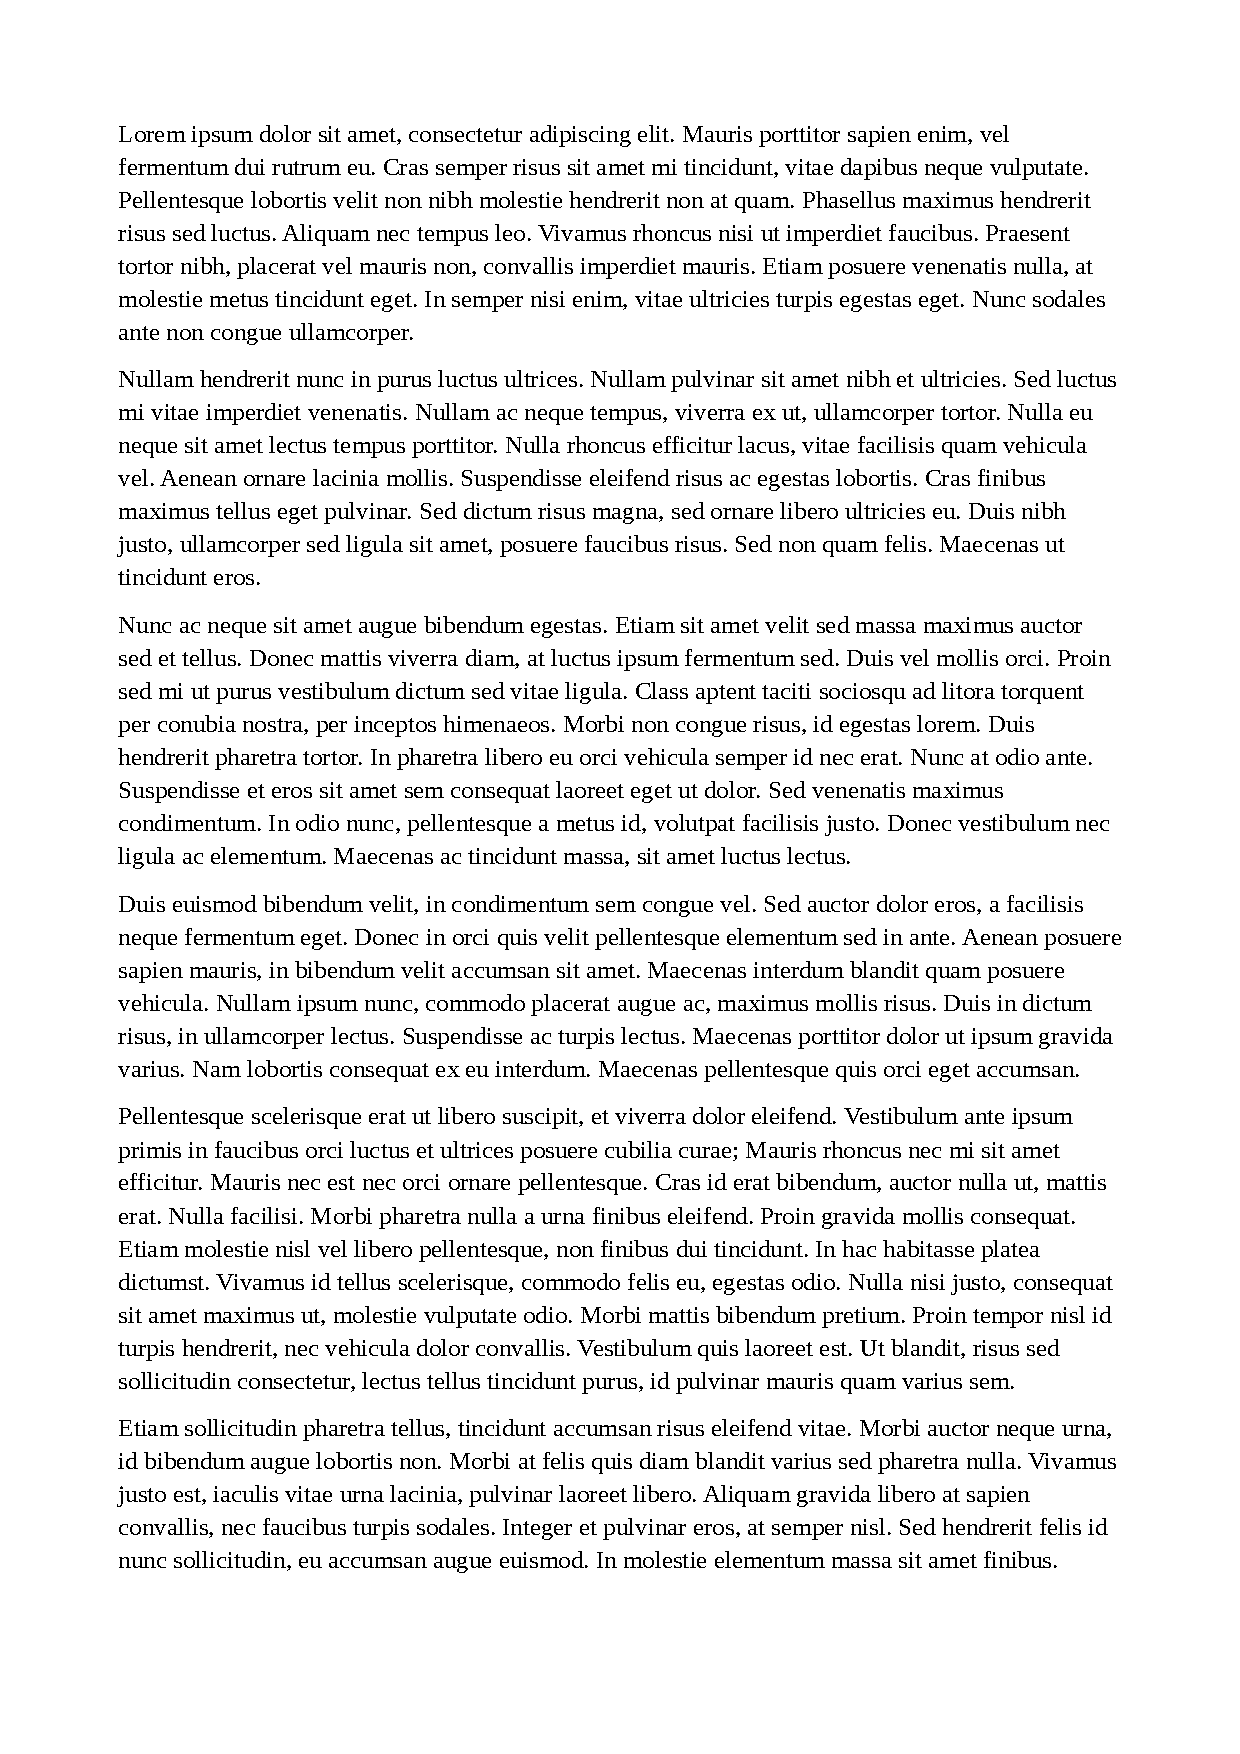
\includepdf[pages={1},scale=0.8,pagecommand=\chapter{Texto Texto Texto Texto}\label{apen:apendiceA}]{appendix/apendiceA}
% \includepdf[pages={2-},scale=0.80,pagecommand={}]{appendix/apendiceA}
